Para diseñar nuestra máquina nos hemos basado en varios proyectos que encontramos en Internet, sobre todo vídeos de gente que ya había intentado hacer máquinas de barajar o repartir cartas. Estos vídeos nos ayudaron a entender diferentes mecanismos, cómo funcionan los rodillos para mover las cartas, cómo repartirlas girando un plato y qué tipo de control es necesario con microcontroladores como Arduino.

En concreto, tomamos como referencia los siguientes proyectos:

\begin{itemize}
    \item Un vídeo donde se analiza una máquina automática de barajado y reparto con un sistema rotatorio \cite{video1}. Este ejemplo nos sirvió para entender cómo sincronizar el motor que expulsa las cartas con el movimiento del plato que gira.

    \item Un proyecto de un creador independiente que muestra una máquina capaz de clasificar y repartir cartas \cite{video2}. Nos fue útil para ver cómo diseñar los rodillos, las guías y por qué es importante usar goma o superficies de alta fricción.

    \item Un modelo más avanzado de dispensador de cartas con rodillos y sensores ópticos \cite{video3}. Este vídeo nos ayudó sobre todo con ideas para evitar que salgan varias cartas a la vez y para ver cómo se pueden calibrar los sensores IR.
\end{itemize}

Aunque estos vídeos fueron un buen punto de partida, no copiamos ningún diseño tal cual. Hemos tenido que adaptar muchas cosas, cambiar medidas, modificar mecanismos y ajustar toda la parte electrónica para que funcionase con nuestro diseño y nuestros componentes. Gracias a estas referencias pudimos comparar varias opciones y crear una solución que se ajustara a los objetivos del proyecto y que fuera lo más fiable posible.

\begin{figure}[H]
    \centering
    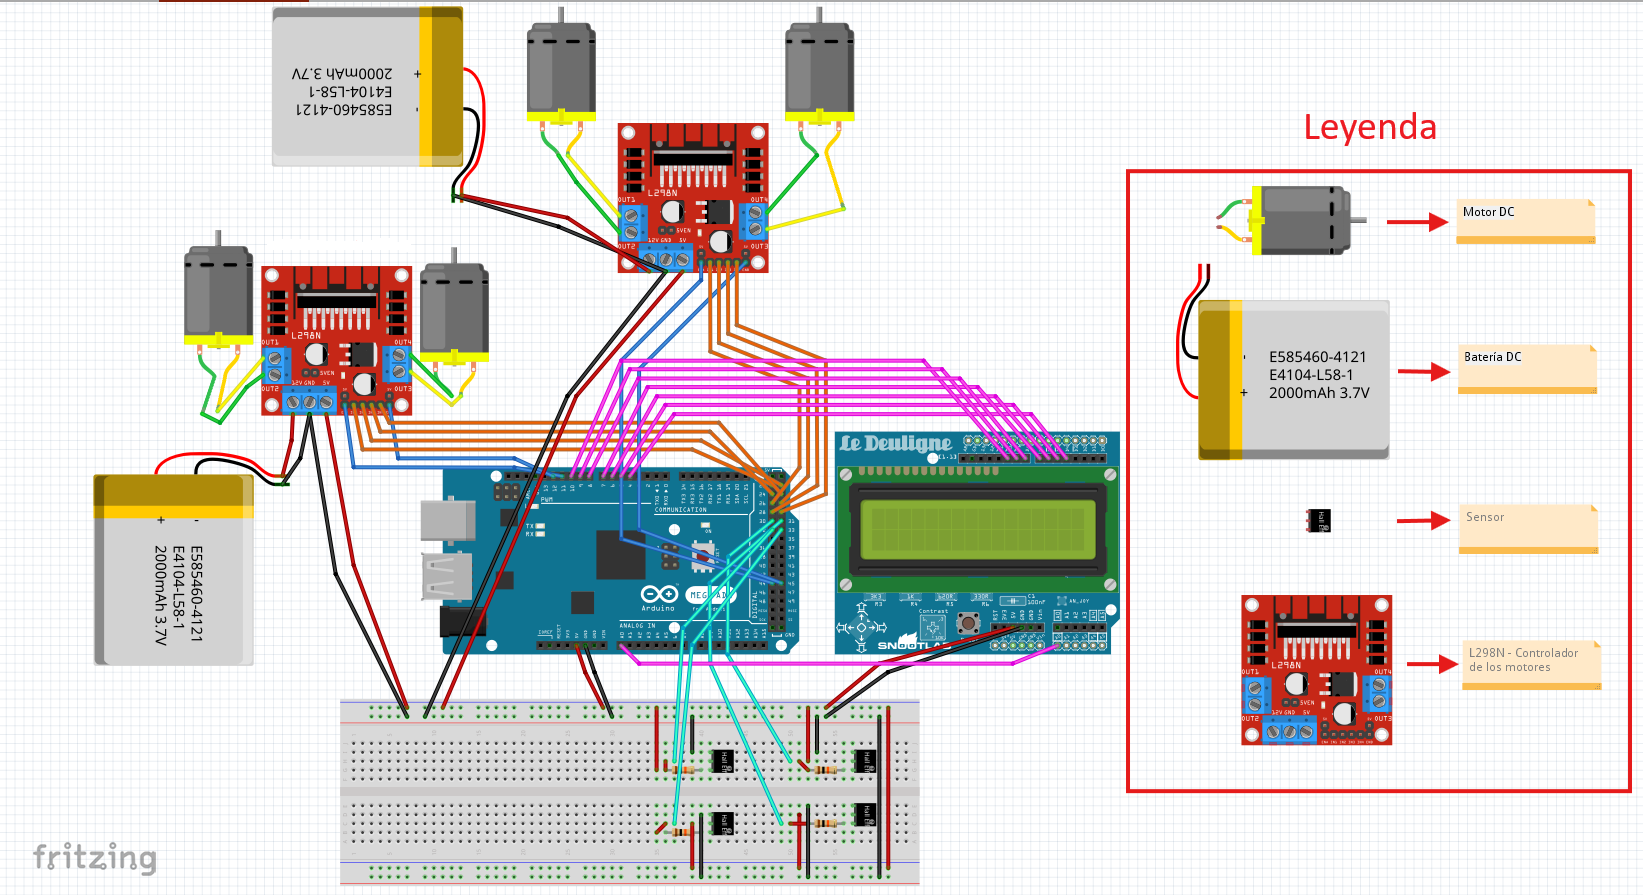
\includegraphics[width=0.75\textwidth]{esquema_final.png}
    \caption{Diseño del esquema eléctrico}
    \label{fig:esquema_electrico}
\end{figure}


\subsection{Diseño Estructural y Modelado CAD}

Para el desarrollo de la estructura física del prototipo \textbf{ELCO-Dealer}, se ha empleado la herramienta de diseño asistido por computadora (CAD) basada en la nube \textbf{OnShape}. Esta plataforma permitió realizar un modelado paramétrico detallado de todos los componentes mecánicos, asegurando la compatibilidad entre las piezas antes de su fabricación.

El elemento central de este diseño es el \textbf{dispensador de cartas}, el cual ha sido optimizado geométricamente para garantizar la separación exacta de las cartas y minimizar la probabilidad de atascos durante el reparto automático. En la Figura \ref{fig:planos_dispensador_onshape} se presentan los planos obtenidos del modelo de OnShape.

\begin{figure}[H]
    \centering
    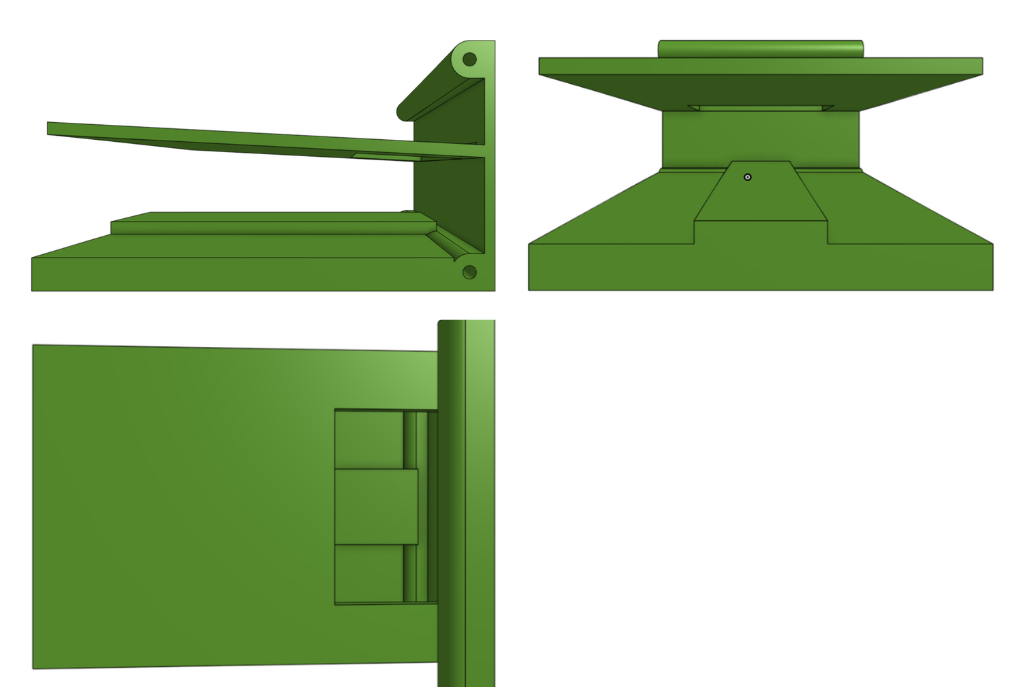
\includegraphics[width=0.75\textwidth]{onhsape repartidor.png}
    \caption{Diseño del repartidor con el programa OnShape}
    \label{fig:planos_dispensador_onshape}
\end{figure}

Para facilitar el reparto multidireccional de los naipes a las distintas posiciones de los jugadores, el diseño integra una plataforma de giro basada en un rodamiento tipo \textbf{Lazy Susan}. Este mecanismo constituye el soporte estructural de la torreta móvil y ha sido optimizado para garantizar una rotación concéntrica suave y con mínima fricción, lo cual es crítico para la precisión del motor de giro. La implementación de este rodamiento es lo que permite el aprovechamiento total del \textbf{anillo colector (Slip Ring)}, posibilitando que el sistema realice rotaciones de 360º de forma continua e infinita sin comprometer la integridad del cableado que alimenta los motores de barajado y reparto. El modelado detallado de este conjunto, inspirado en sistemas de giro motorizados eficientes, se presenta a continuación:

\begin{figure}[H]
    \centering
    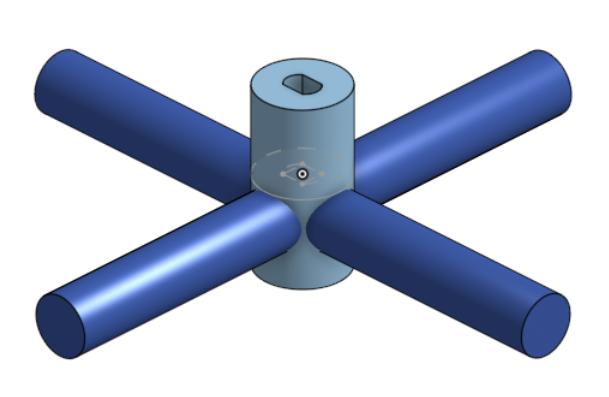
\includegraphics[width=0.5\textwidth]{lazy susan.png}
    \caption{Diseño de la plataforma de giro Lazy Susan con el programa OnShape}
    \label{fig:planos_dispensador}
\end{figure}

